\chapter{جمع‌بندي و نتيجه‌گيري و پیشنهادات}

\section{
بررسی کاهش بعد نرمال
$(\alpha=2)$
به دو بعد
}

\subsection{جداول مقایسه عملکرد خوشه‌بندی}

\begin{table}[H]
\centering\rowcolors{2}{gray!6}{white}
\caption{
عملکرد تصویر تصادفی نرمال برای کاهش بعد به دو بعد
}
\bigskip
\begin{latin}
\begin{tabular}{lrrr}
\hiderowcolors
\toprule
Dataset & $ARI_p$ & $ARI_d$ & $C_e$\\
\midrule
\showrowcolors
Thyroid & 0.5831656 & 0.3989981 & -18\\
Iris & 0.6201352 & 0.4710315 & -15\\
Diabetes & 0.3801662 & 0.3647537 & -2\\
Swiss Banknotes & 0.8456292 & 0.3880871 & -46\\
Seeds & 0.7732937 & 0.4482112 & -33\\
\addlinespace
Crabs & 0.0481402 & 0.0439549 & 0\\
Mice Protein Expression & 0.1316117 & 0.0657659 & -7\\
\bottomrule
\end{tabular}
\end{latin}
\rowcolors{2}{white}{white}
\end{table}


\subsection{نمودار فراوانی عملکرد خوشه‌بندی}


\begin{center}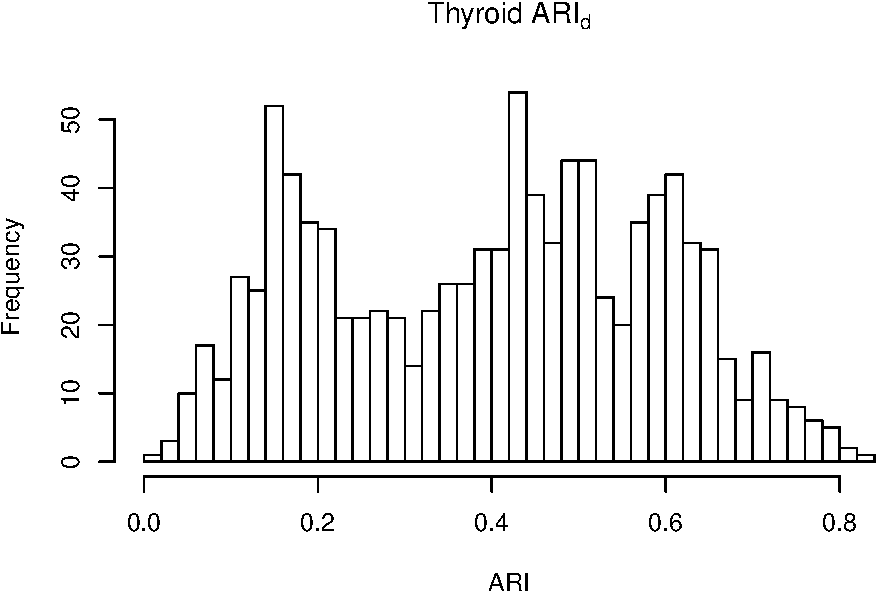
\includegraphics[width=1\linewidth]{Report_files/figure-latex/unnamed-chunk-3-1} \end{center}

\begin{center}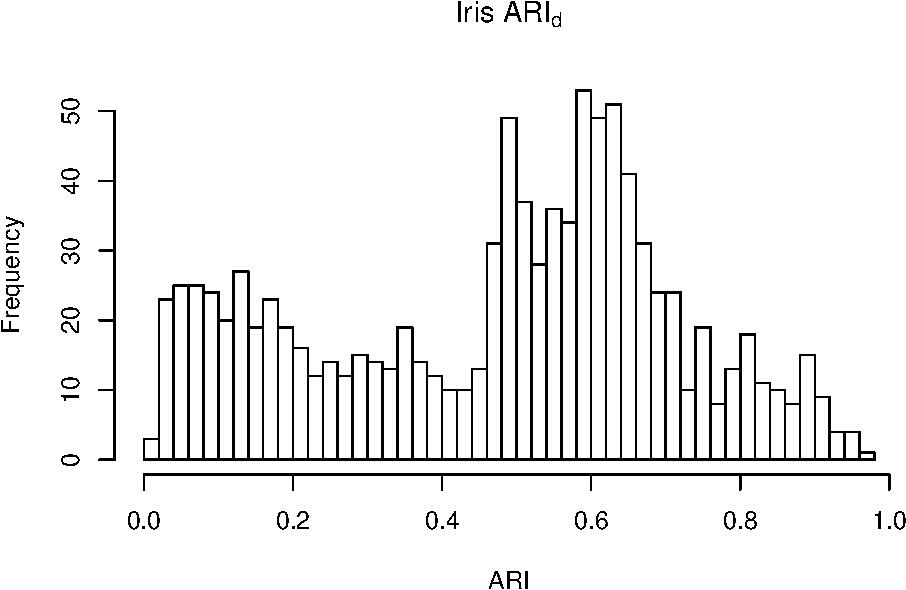
\includegraphics[width=1\linewidth]{Report_files/figure-latex/unnamed-chunk-3-2} \end{center}

\begin{center}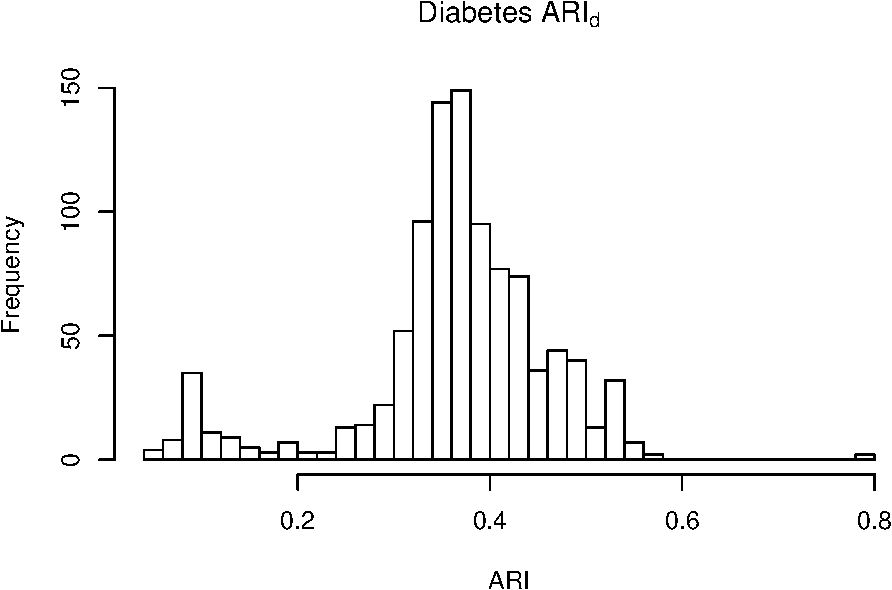
\includegraphics[width=1\linewidth]{Report_files/figure-latex/unnamed-chunk-3-3} \end{center}

\begin{center}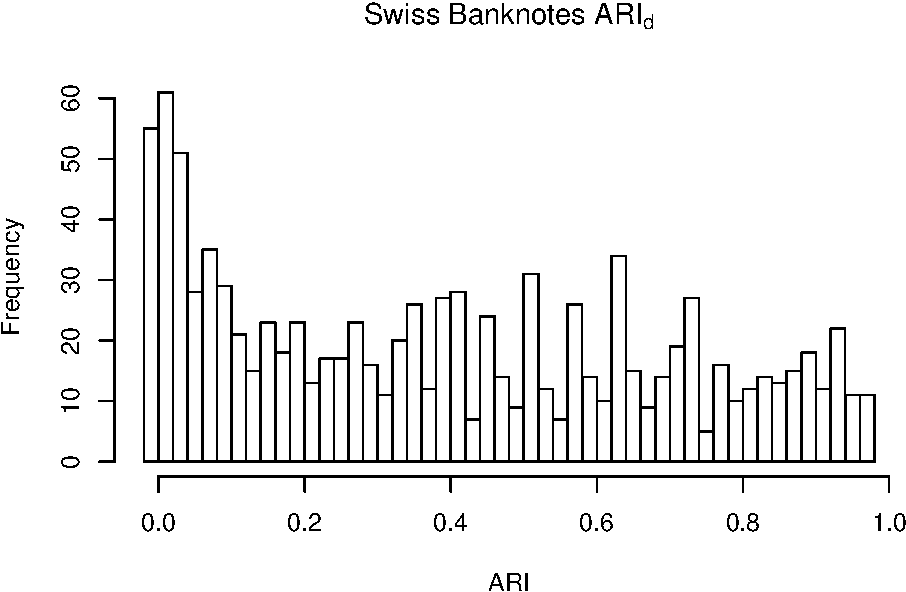
\includegraphics[width=1\linewidth]{Report_files/figure-latex/unnamed-chunk-3-4} \end{center}

\begin{center}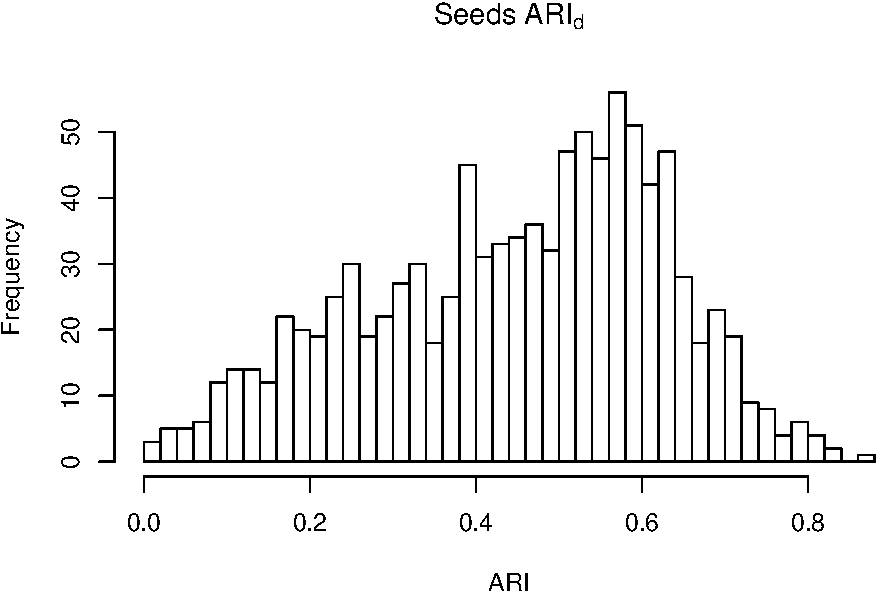
\includegraphics[width=1\linewidth]{Report_files/figure-latex/unnamed-chunk-3-5} \end{center}

\begin{center}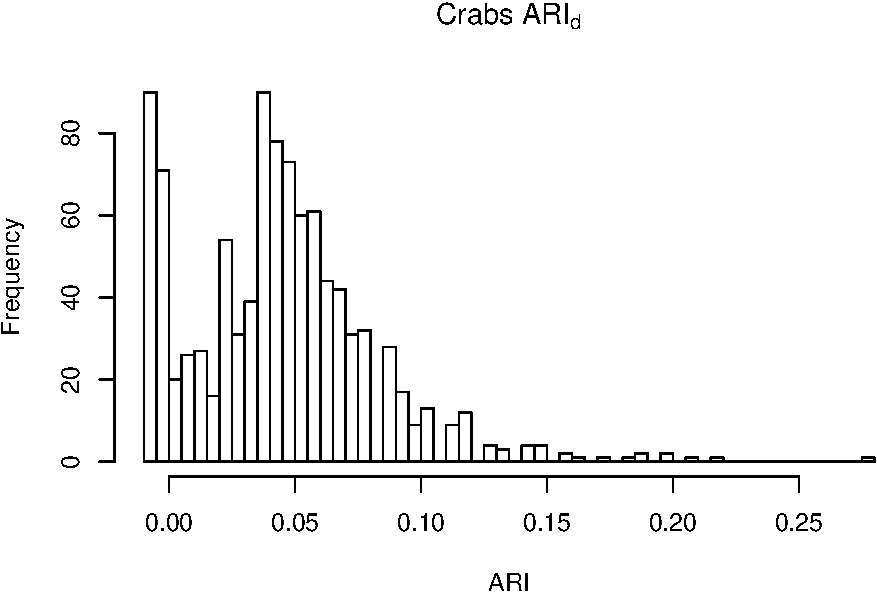
\includegraphics[width=1\linewidth]{Report_files/figure-latex/unnamed-chunk-3-6} \end{center}

\begin{center}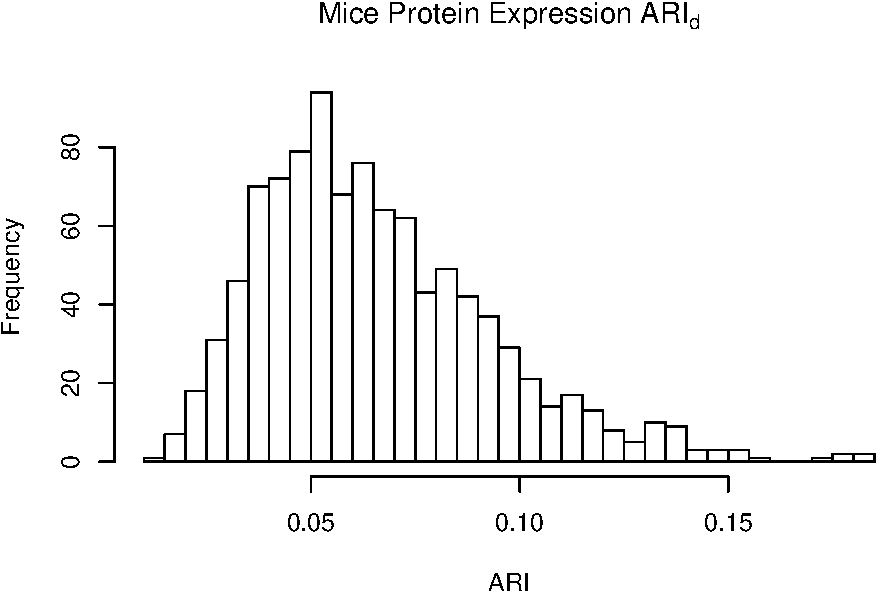
\includegraphics[width=1\linewidth]{Report_files/figure-latex/unnamed-chunk-3-7} \end{center}








\section{نتایج برای کاهش بعد نرمال به سه بعد}

\subsection{جداول مقایسه عملکرد خوشه‌بندی}


\begin{table}[H]
\caption{
عملکرد تصویر تصادفی نرمال برای کاهش بعد به سه بعد
}
\bigskip
\centering\rowcolors{2}{gray!6}{white}
\begin{latin}
\begin{tabular}{lrrr}
\hiderowcolors
\toprule
Dataset & $ARI_p$ & $ARI_d$ & $C_e$\\
\midrule
\showrowcolors
Thyroid & 0.5831656 & 0.4344288 & -15\\
Iris & 0.6201352 & 0.5359746 & -8\\
Diabetes & 0.3801662 & 0.3805076 & 0\\
Swiss Banknotes & 0.8456292 & 0.4714675 & -37\\
Seeds & 0.7732937 & 0.5299329 & -24\\
\addlinespace
Mice Protein Expression & 0.1316575 & 0.0814613 & -5\\
Crabs & 0.0481402 & 0.0485252 & 0\\
\bottomrule
\end{tabular}
\end{latin}
\rowcolors{2}{white}{white}
\end{table}


\subsection{نمودار فراوانی عملکرد خوشه‌بندی}


\begin{center}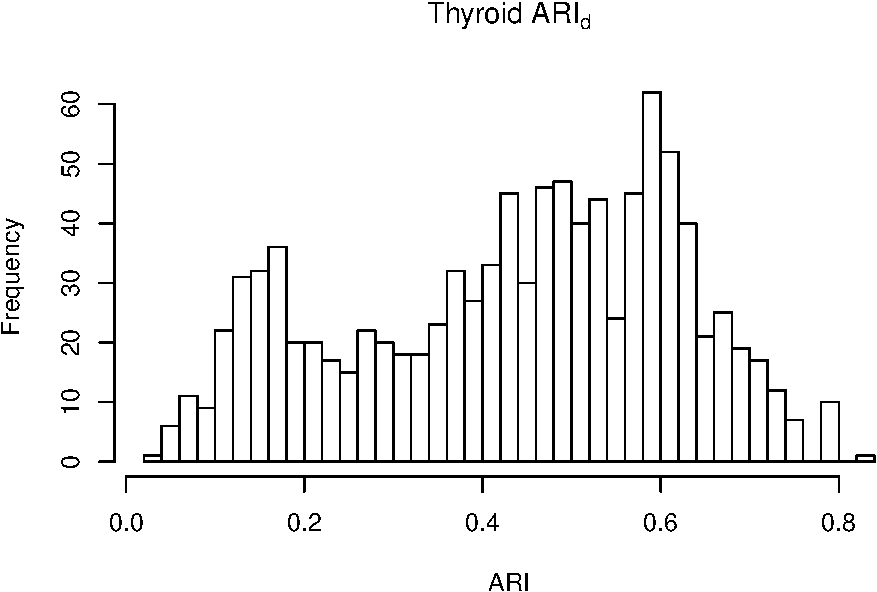
\includegraphics[width=1\linewidth]{Report_files/figure-latex/unnamed-chunk-6-1} \end{center}

\begin{center}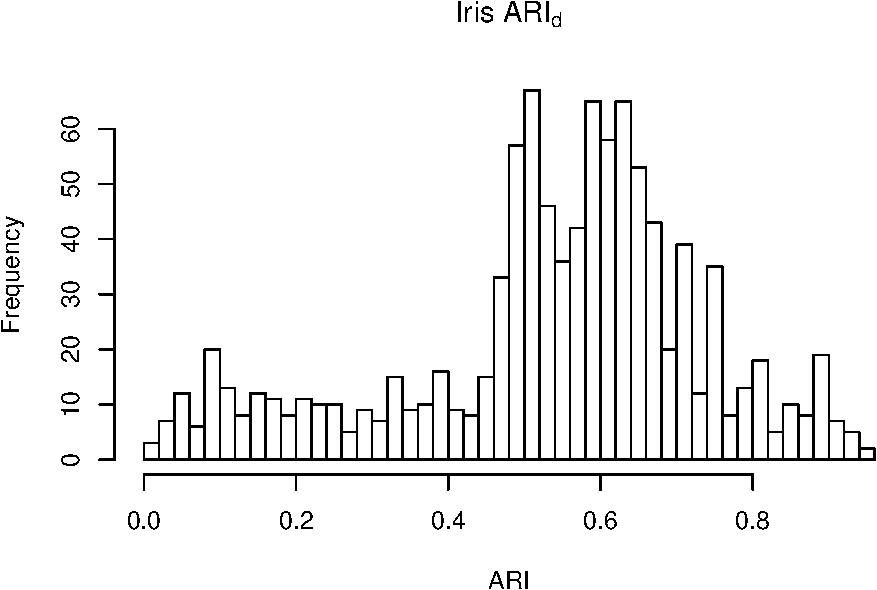
\includegraphics[width=1\linewidth]{Report_files/figure-latex/unnamed-chunk-6-2} \end{center}

\begin{center}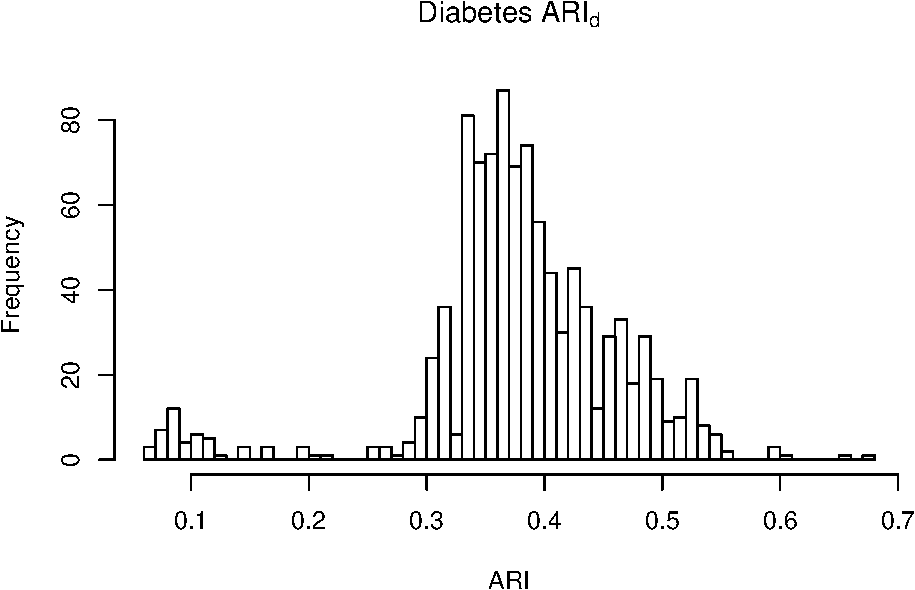
\includegraphics[width=1\linewidth]{Report_files/figure-latex/unnamed-chunk-6-3} \end{center}

\begin{center}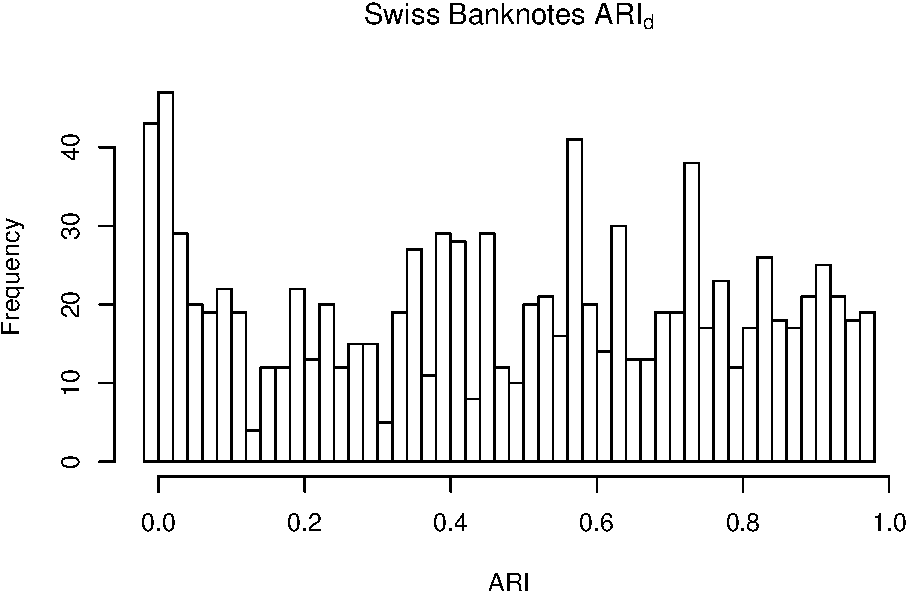
\includegraphics[width=1\linewidth]{Report_files/figure-latex/unnamed-chunk-6-4} \end{center}

\begin{center}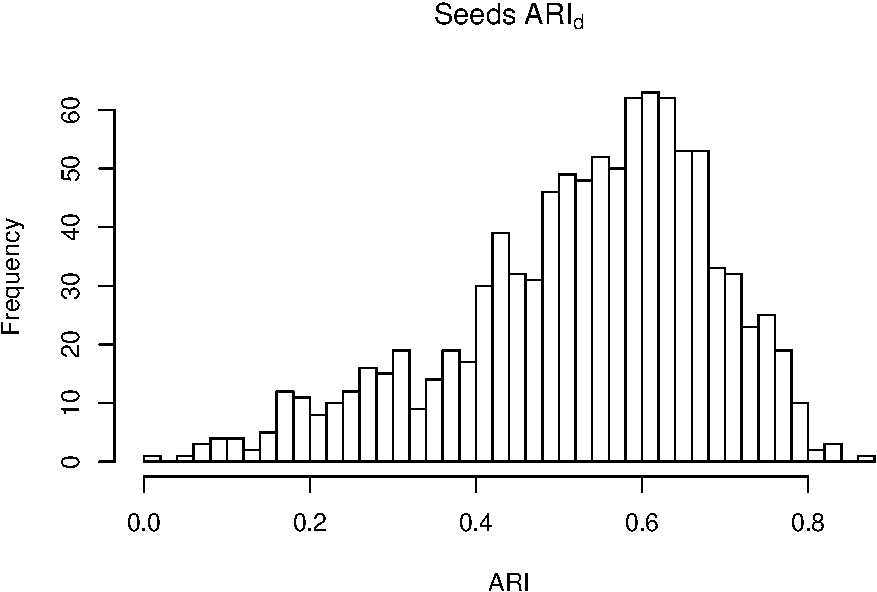
\includegraphics[width=1\linewidth]{Report_files/figure-latex/unnamed-chunk-6-5} \end{center}

\begin{center}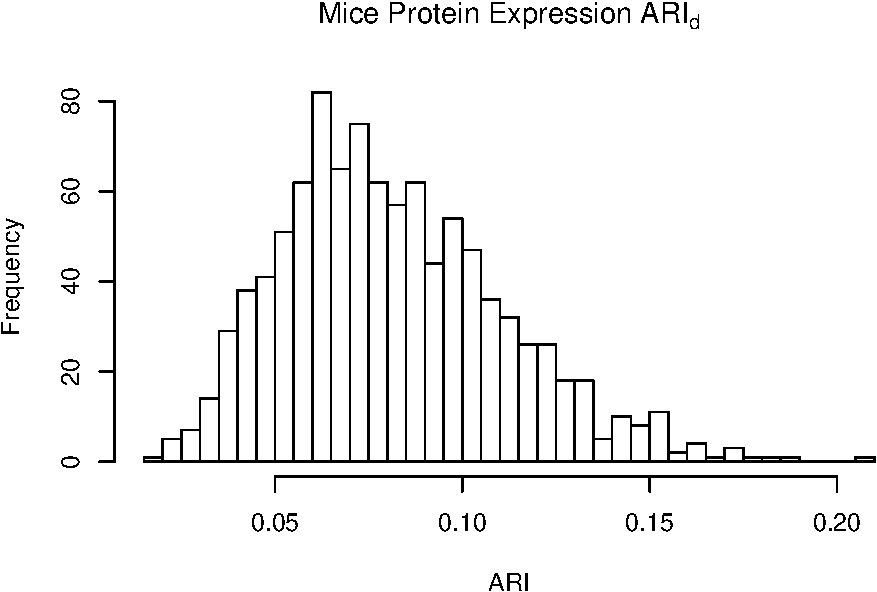
\includegraphics[width=1\linewidth]{Report_files/figure-latex/unnamed-chunk-6-6} \end{center}

\begin{center}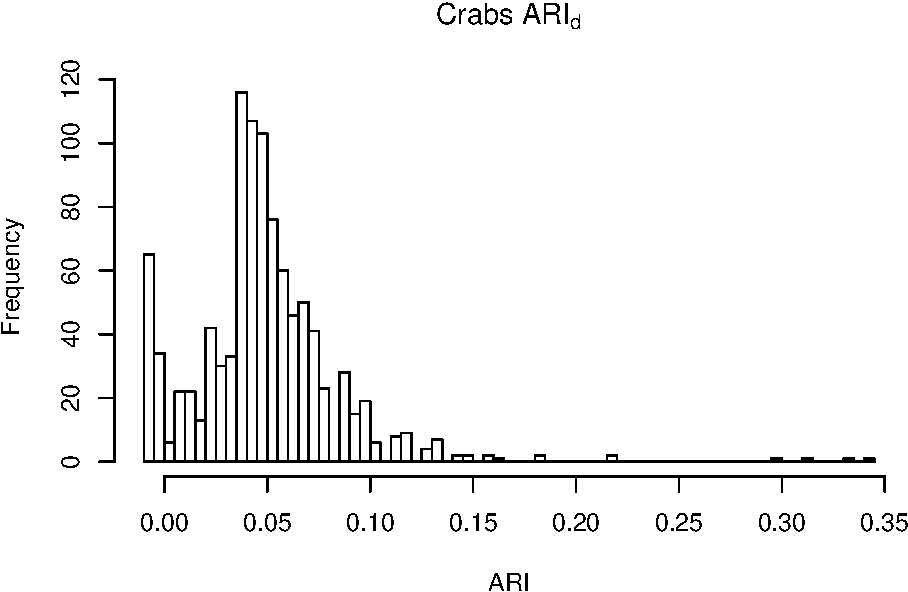
\includegraphics[width=1\linewidth]{Report_files/figure-latex/unnamed-chunk-6-7} \end{center}








\section{
نتایج برای کاهش بعد کوشی 
$(\alpha = 1)$
به دو بعد
}

\subsection{جداول مقایسه عملکرد خوشه‌بندی}


\begin{table}[H]
\caption{
عملکرد تصویر تصادفی کوشی برای کاهش بعد به دو بعد
}
\bigskip
\centering\rowcolors{2}{gray!6}{white}
\begin{latin}
\begin{tabular}{lrrr}
\hiderowcolors
\toprule
Dataset & $ARI_p$ & $ARI_d$ & $C_e$\\
\midrule
\showrowcolors
Thyroid & 0.5831656 & 0.3559301 & -23\\
Iris & 0.6201352 & 0.5078172 & -11\\
Diabetes & 0.3801662 & 0.3341399 & -5\\
Swiss Banknotes & 0.8456292 & 0.4011119 & -44\\
Seeds & 0.7732937 & 0.4488349 & -32\\
\addlinespace
Mice Protein Expression & 0.1317342 & 0.0592468 & -7\\
Crabs & 0.0481402 & 0.0469365 & 0\\
\bottomrule
\end{tabular}
\end{latin}
\rowcolors{2}{white}{white}
\end{table}


\subsection{نمودار فراوانی عملکرد خوشه‌بندی}


\begin{center}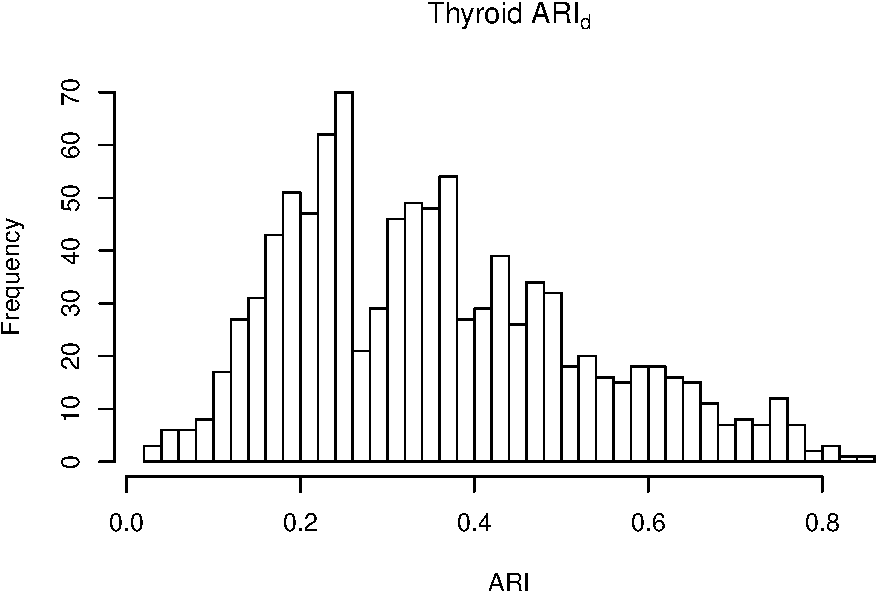
\includegraphics[width=1\linewidth]{Report_files/figure-latex/unnamed-chunk-9-1} \end{center}

\begin{center}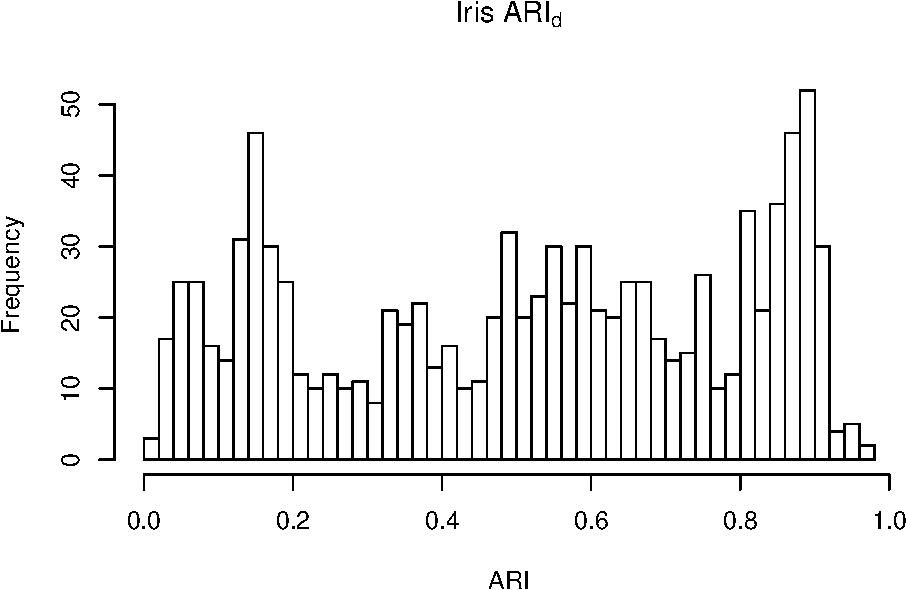
\includegraphics[width=1\linewidth]{Report_files/figure-latex/unnamed-chunk-9-2} \end{center}

\begin{center}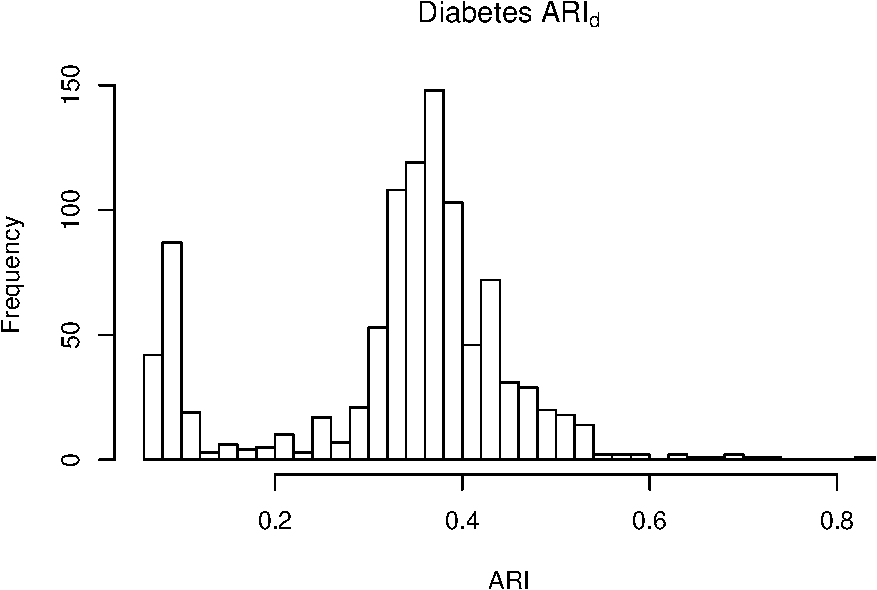
\includegraphics[width=1\linewidth]{Report_files/figure-latex/unnamed-chunk-9-3} \end{center}

\begin{center}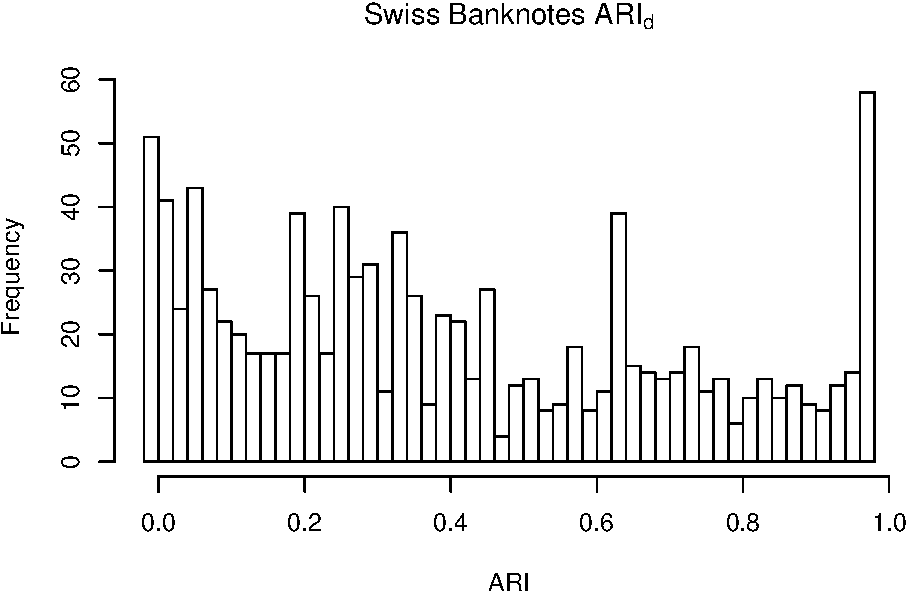
\includegraphics[width=1\linewidth]{Report_files/figure-latex/unnamed-chunk-9-4} \end{center}

\begin{center}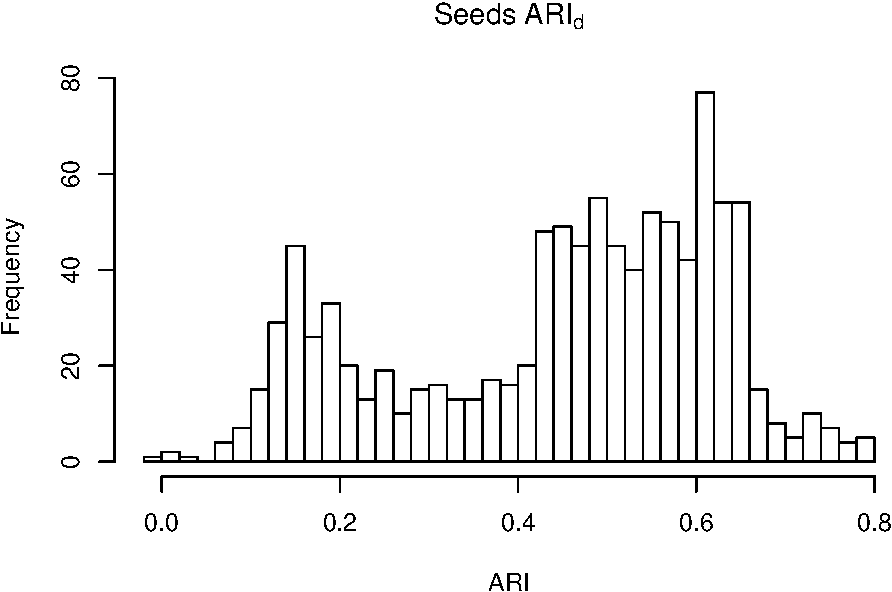
\includegraphics[width=1\linewidth]{Report_files/figure-latex/unnamed-chunk-9-5} \end{center}

\begin{center}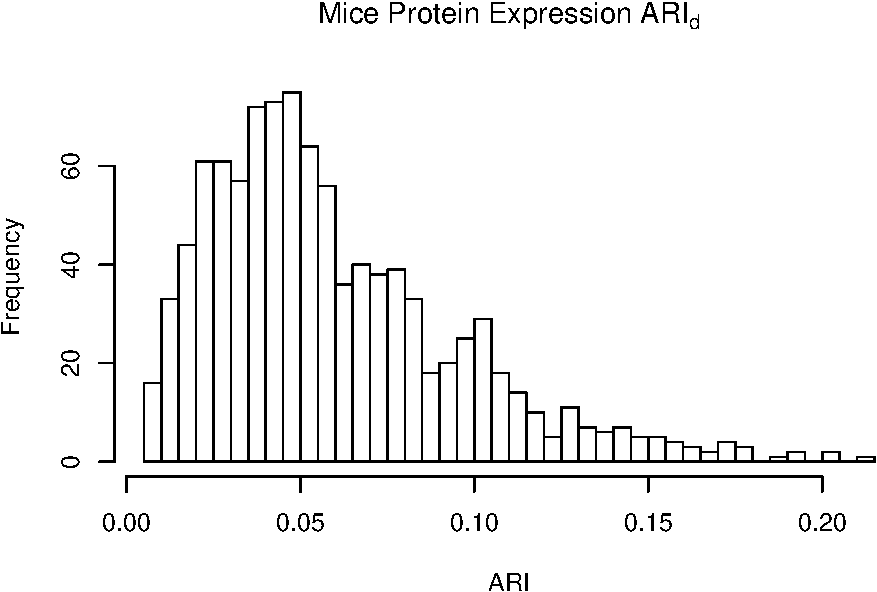
\includegraphics[width=1\linewidth]{Report_files/figure-latex/unnamed-chunk-9-6} \end{center}

\begin{center}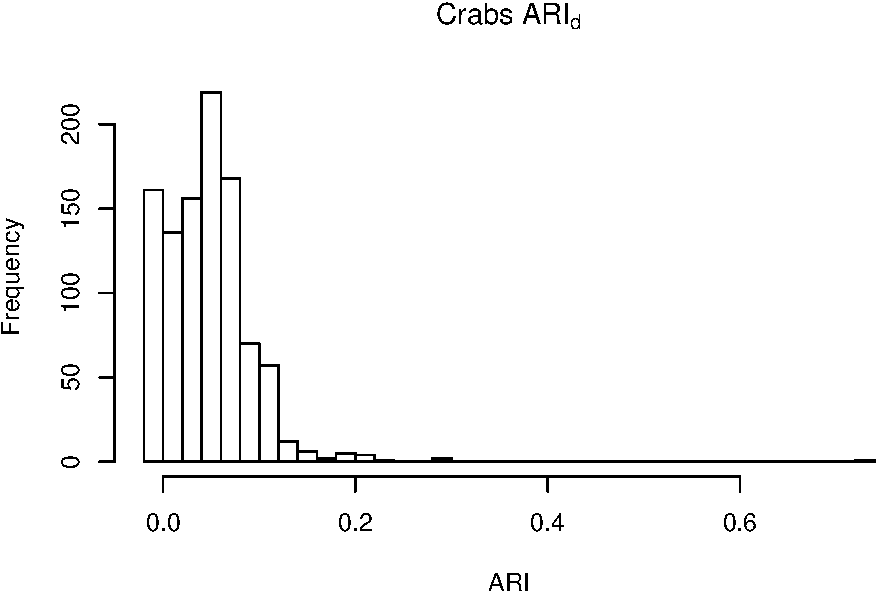
\includegraphics[width=1\linewidth]{Report_files/figure-latex/unnamed-chunk-9-7} \end{center}






\section{نتایج برای کاهش بعد کوشی به سه بعد}

\subsection{جداول مقایسه عملکرد خوشه‌بندی}

\begin{table}[H]
\caption{
عملکرد تصویر تصادفی کوشی برای کاهش بعد به سه بعد
}
\bigskip
\centering\rowcolors{2}{gray!6}{white}
\begin{latin}
\begin{tabular}{lrrr}
\hiderowcolors
\toprule
Dataset & $ARI_p$ & $ARI_d$ & $C_e$\\
\midrule
\showrowcolors
Thyroid & 0.5831656 & 0.3658900 & -22\\
Iris & 0.6201352 & 0.5441285 & -8\\
Diabetes & 0.3801662 & 0.3460760 & -3\\
Swiss Banknotes & 0.8456292 & 0.4330544 & -41\\
Seeds & 0.7732937 & 0.4697687 & -30\\
\addlinespace
Mice Protein Expression & 0.1317362 & 0.0659775 & -7\\
Crabs & 0.0481402 & 0.0452313 & 0\\
\bottomrule
\end{tabular}
\end{latin}
\rowcolors{2}{white}{white}
\end{table}


\subsection{نمودار فراوانی عملکرد خوشه‌بندی}

\begin{center}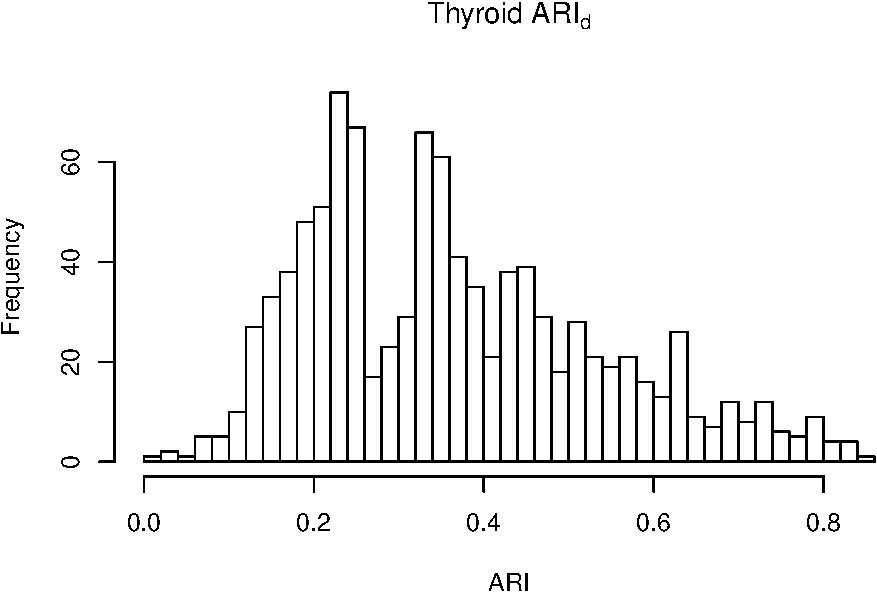
\includegraphics[width=1\linewidth]{Report_files/figure-latex/unnamed-chunk-12-1} \end{center}

\begin{center}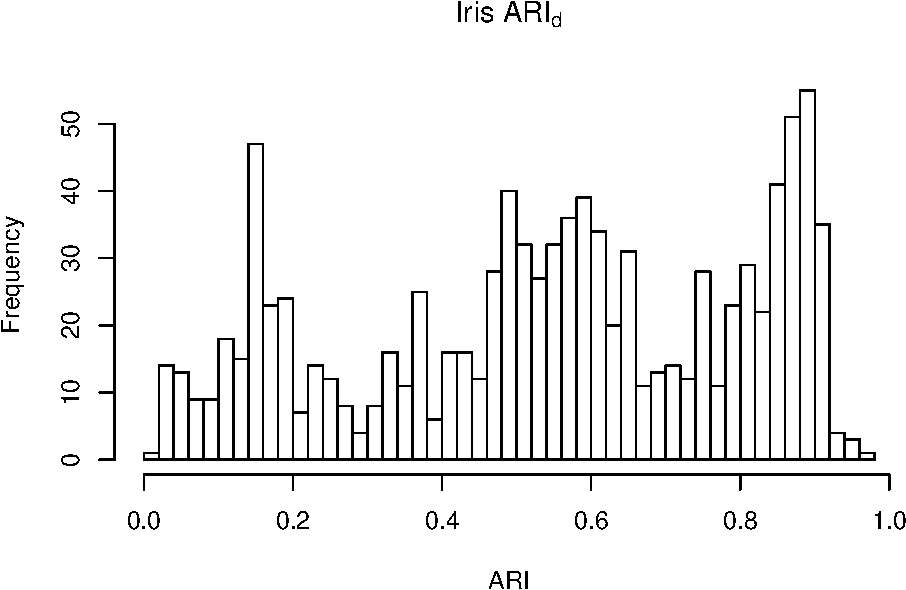
\includegraphics[width=1\linewidth]{Report_files/figure-latex/unnamed-chunk-12-2} \end{center}

\begin{center}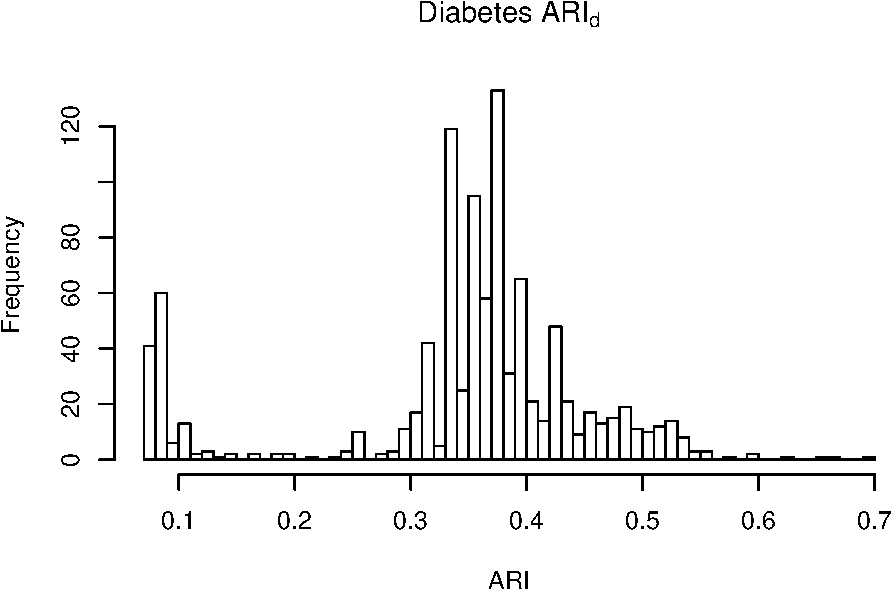
\includegraphics[width=1\linewidth]{Report_files/figure-latex/unnamed-chunk-12-3} \end{center}

\begin{center}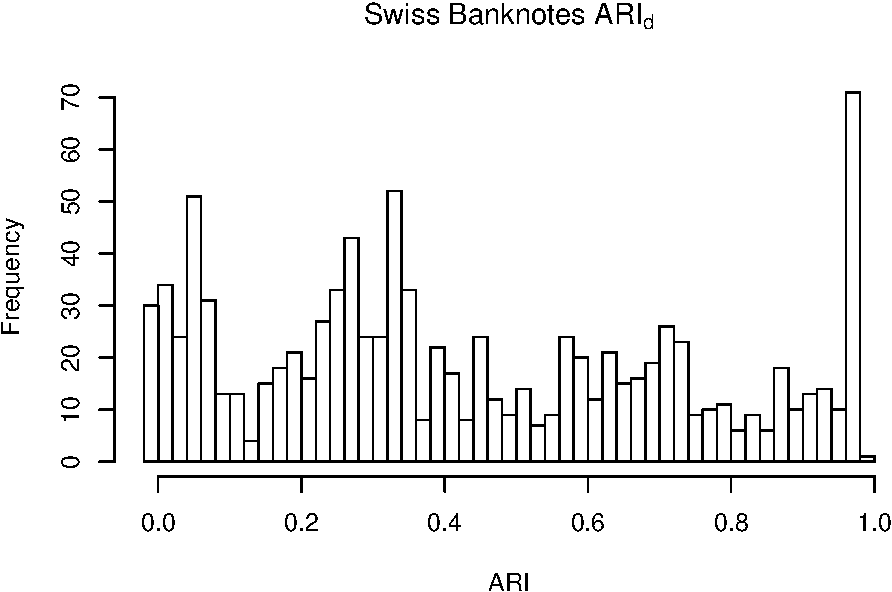
\includegraphics[width=1\linewidth]{Report_files/figure-latex/unnamed-chunk-12-4} \end{center}

\begin{center}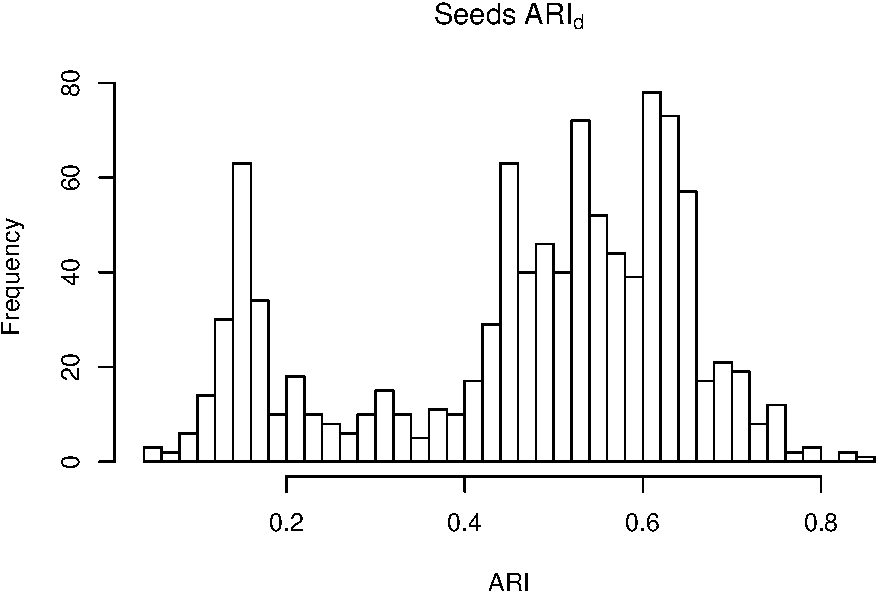
\includegraphics[width=1\linewidth]{Report_files/figure-latex/unnamed-chunk-12-5} \end{center}

\begin{center}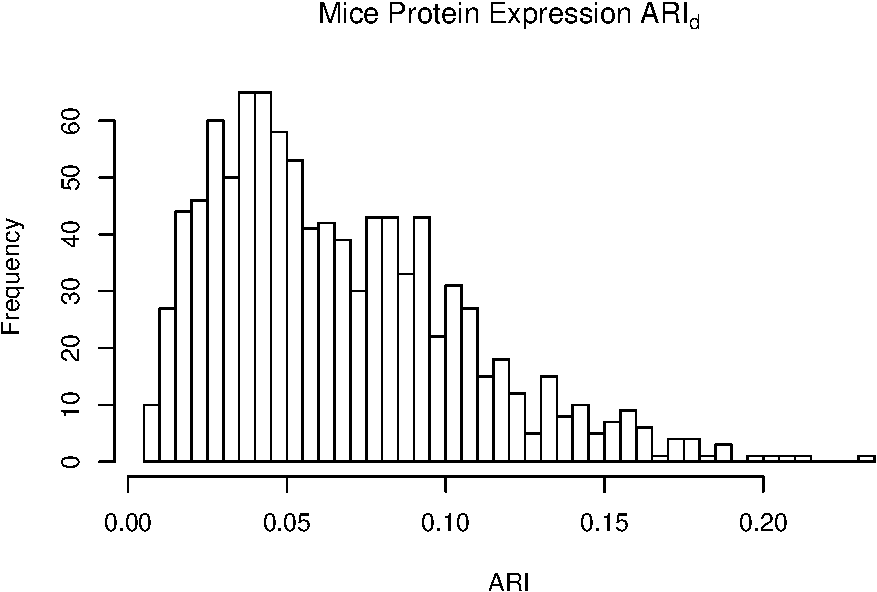
\includegraphics[width=1\linewidth]{Report_files/figure-latex/unnamed-chunk-12-6} \end{center}

\begin{center}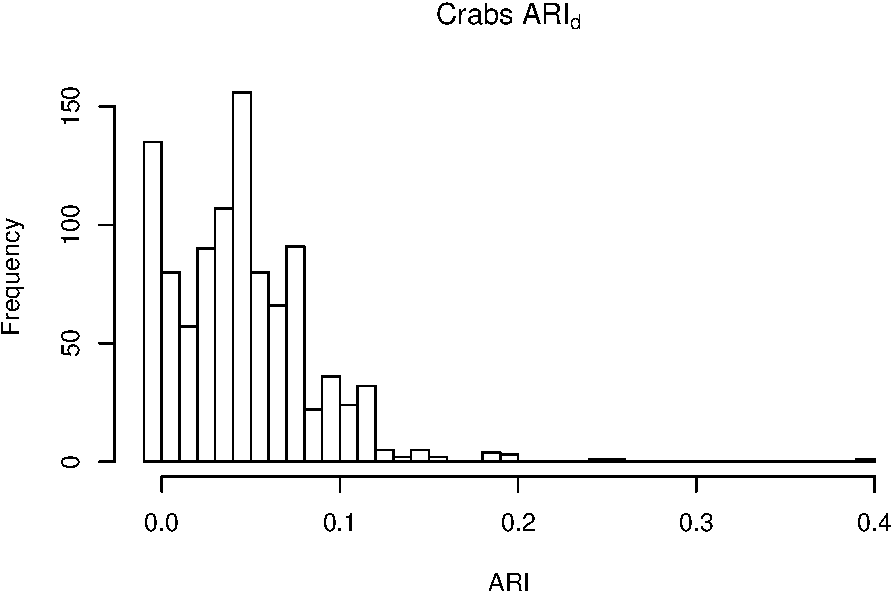
\includegraphics[width=1\linewidth]{Report_files/figure-latex/unnamed-chunk-12-7} \end{center}


\section{
نتایج برای کاهش بعد گسسته $s=2$ به دو بعد
}

\subsection{جداول مقایسه عملکرد خوشه‌بندی}

\begin{table}[H]
\caption{
عملکرد تصویر تصادفی گسسته با
$s=1$
برای کاهش بعد به دو بعد
}
\centering\rowcolors{2}{gray!6}{white}
\begin{latin}
\begin{tabular}{lrrr}
\hiderowcolors
\toprule
Dataset & $ARI_p$ & $ARI_d$ & $C_e$\\
\midrule
\showrowcolors
Thyroid & 0.5831656 & 0.4016237 & -18\\
Iris & 0.6201352 & 0.4890477 & -13\\
Diabetes & 0.3801662 & 0.3515435 & -3\\
Swiss Banknotes & 0.8456292 & 0.4012454 & -44\\
Seeds & 0.7732937 & 0.4459104 & -33\\
\addlinespace
Mice Protein Expression & 0.1314435 & 0.0647088 & -7\\
Crabs & 0.0481402 & 0.0467305 & 0\\
\bottomrule
\end{tabular}
\end{latin}
\rowcolors{2}{white}{white}
\end{table}

\subsection{نمودار فراوانی عملکرد خوشه‌بندی}


\begin{center}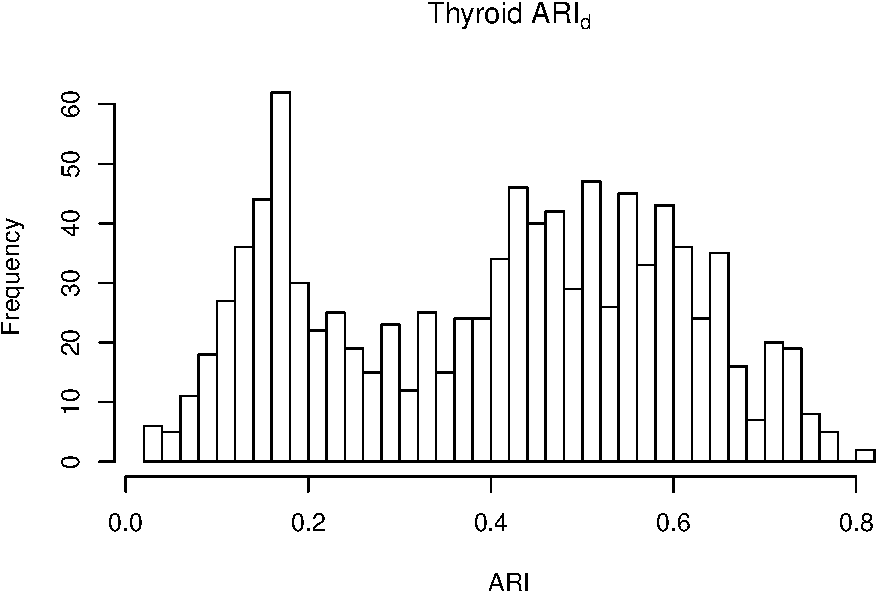
\includegraphics[width=1\linewidth]{Report_files/figure-latex/unnamed-chunk-15-1} \end{center}

\begin{center}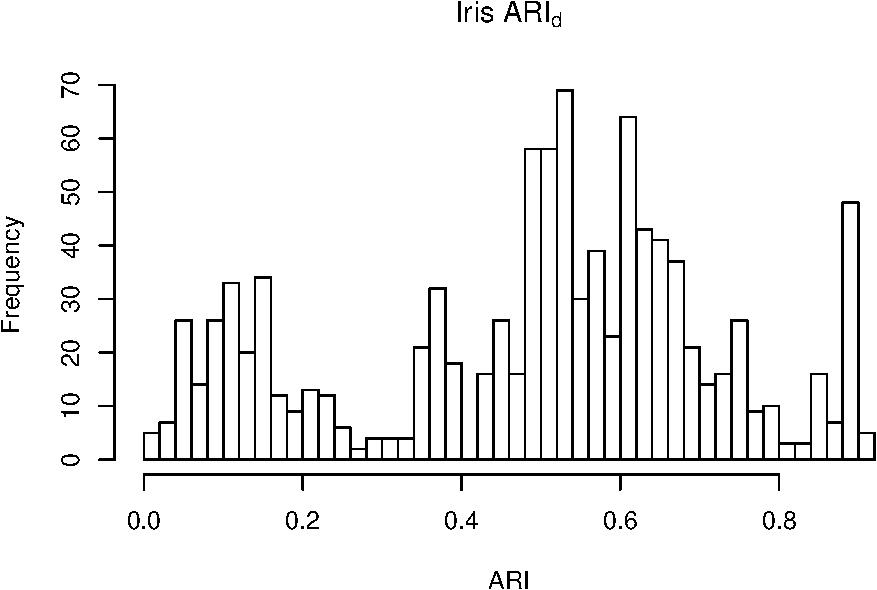
\includegraphics[width=1\linewidth]{Report_files/figure-latex/unnamed-chunk-15-2} \end{center}

\begin{center}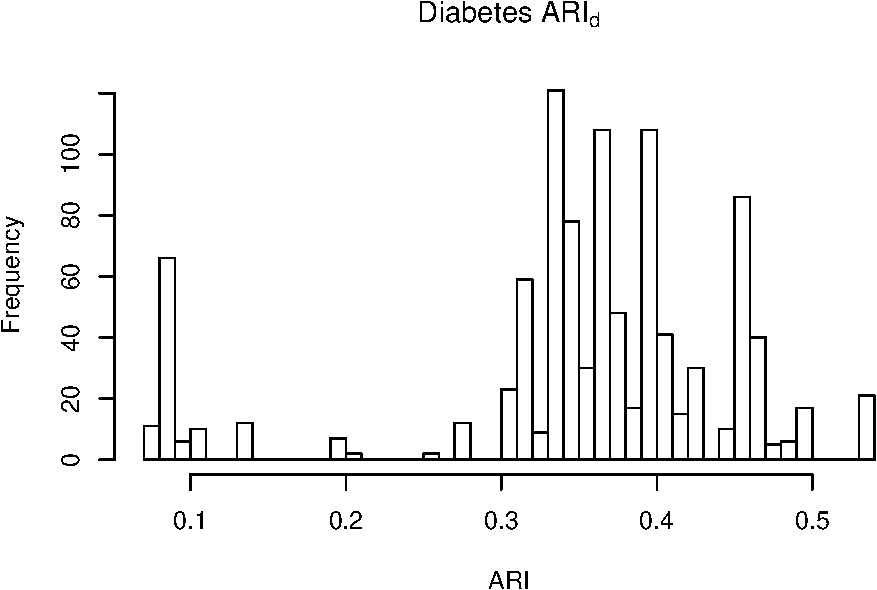
\includegraphics[width=1\linewidth]{Report_files/figure-latex/unnamed-chunk-15-3} \end{center}

\begin{center}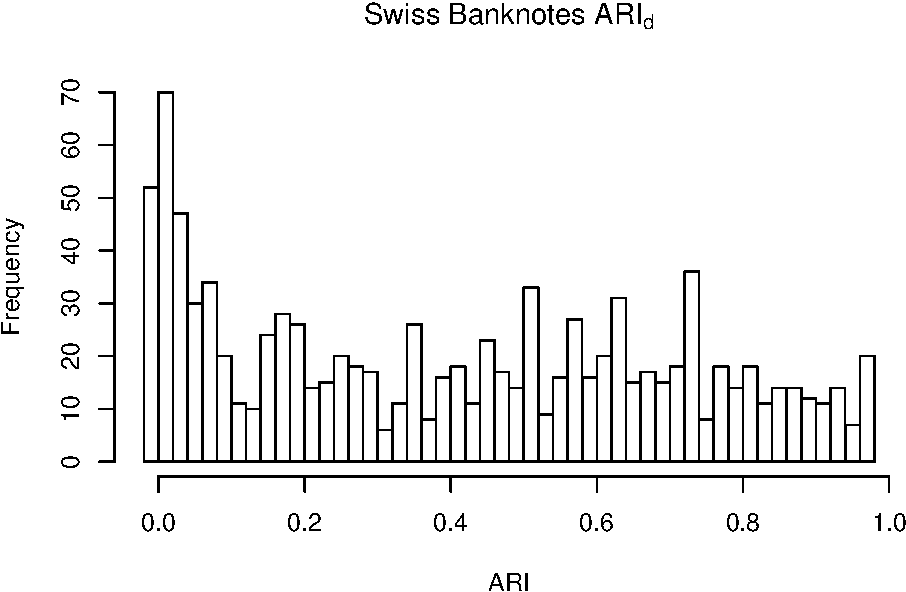
\includegraphics[width=1\linewidth]{Report_files/figure-latex/unnamed-chunk-15-4} \end{center}

\begin{center}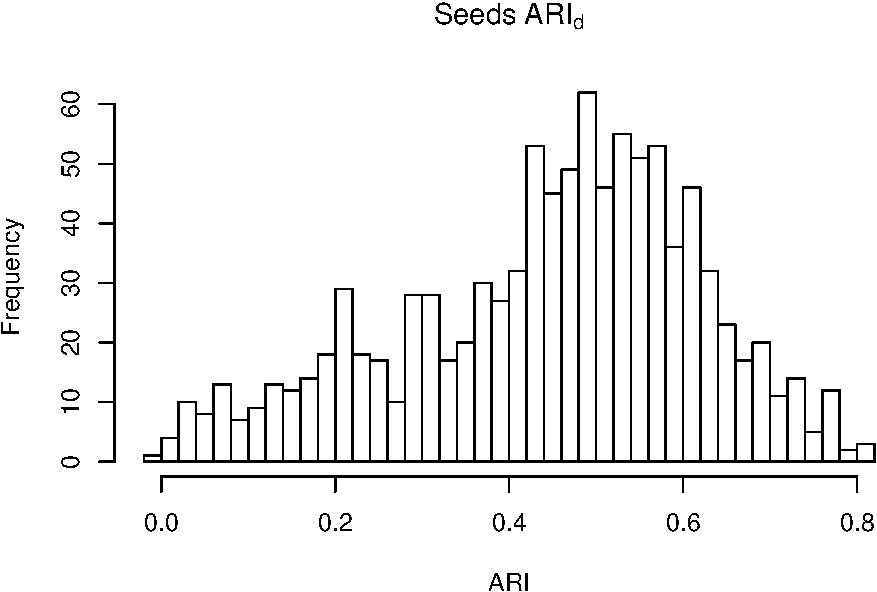
\includegraphics[width=1\linewidth]{Report_files/figure-latex/unnamed-chunk-15-5} \end{center}

\begin{center}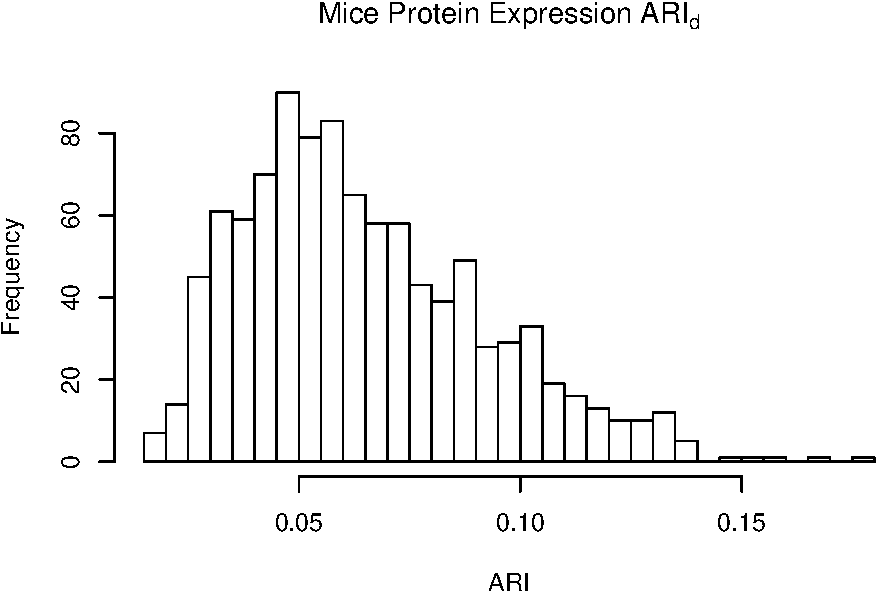
\includegraphics[width=1\linewidth]{Report_files/figure-latex/unnamed-chunk-15-6} \end{center}

\begin{center}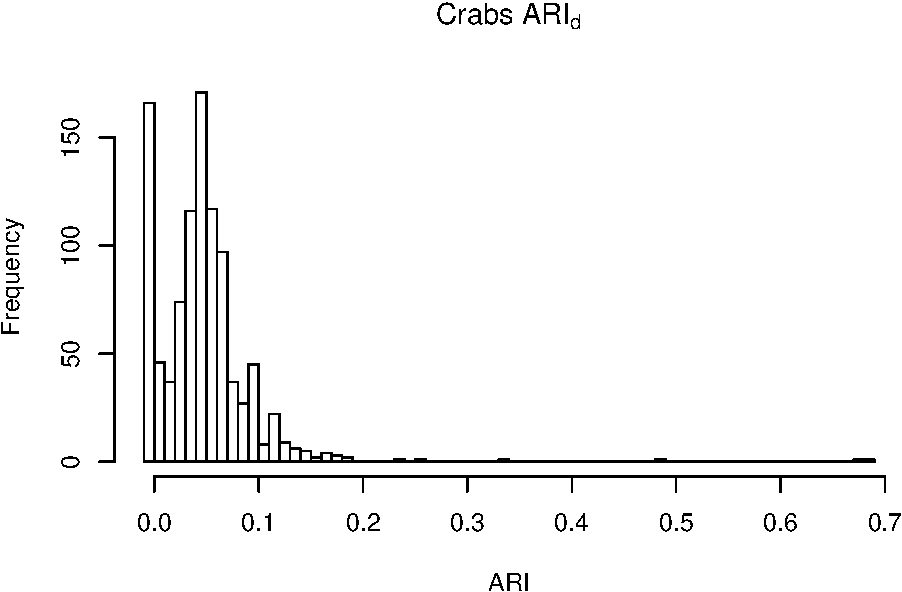
\includegraphics[width=1\linewidth]{Report_files/figure-latex/unnamed-chunk-15-7} \end{center}


\section{
نتایج برای کاهش بعد گسسته $s=2$ به سه بعد
}

\subsection{جداول مقایسه عملکرد خوشه‌بندی}

\begin{table}[H]
\caption{
عملکرد تصویر تصادفی گسسته با 
$s=2$
برای کاهش بعد به سه بعد
}
\centering\rowcolors{2}{gray!6}{white}
\begin{latin}
\begin{tabular}{lrrr}
\hiderowcolors
\toprule
Dataset & $ARI_p$ & $ARI_d$ & $C_e$\\
\midrule
\showrowcolors
Thyroid & 0.5831656 & 0.4386178 & -14\\
Iris & 0.6201352 & 0.5410759 & -8\\
Diabetes & 0.3801662 & 0.3735668 & -1\\
Swiss Banknotes & 0.8456292 & 0.4881694 & -36\\
Seeds & 0.7732937 & 0.5289697 & -24\\
\addlinespace
Mice Protein Expression & 0.1314406 & 0.0798832 & -5\\
Crabs & 0.0481402 & 0.0463655 & 0\\
\bottomrule
\end{tabular}
\end{latin}
\rowcolors{2}{white}{white}
\end{table}


\subsection{نمودار فراوانی عملکرد خوشه‌بندی}


\begin{center}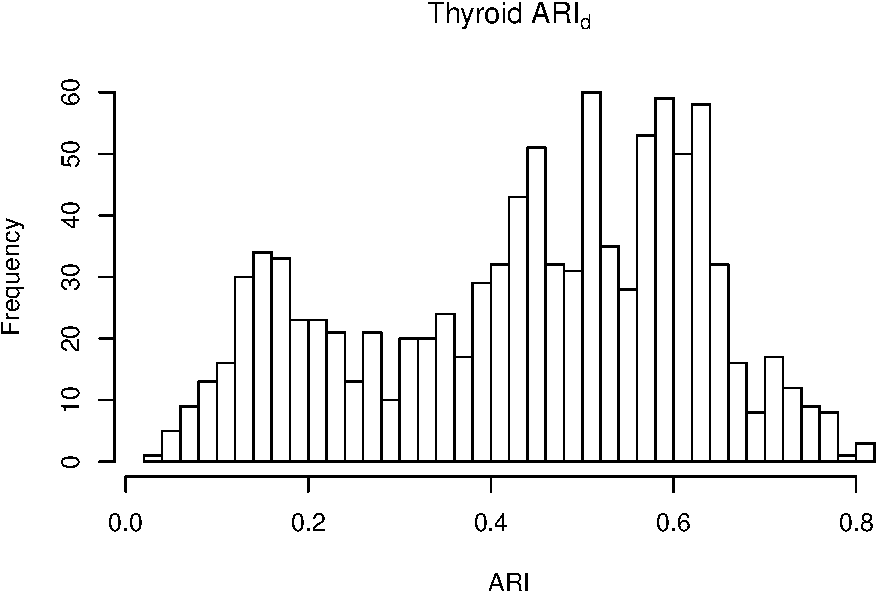
\includegraphics[width=1\linewidth]{Report_files/figure-latex/unnamed-chunk-18-1} \end{center}

\begin{center}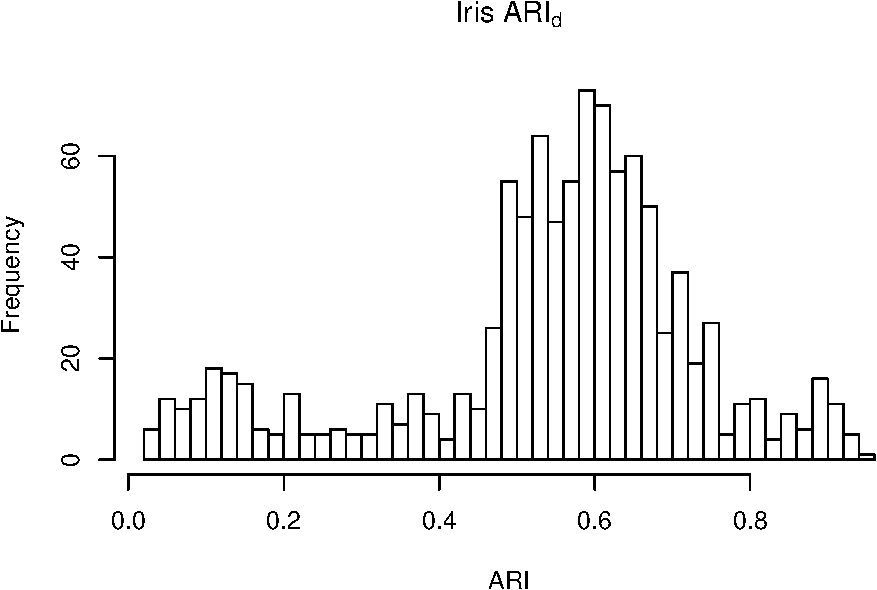
\includegraphics[width=1\linewidth]{Report_files/figure-latex/unnamed-chunk-18-2} \end{center}

\begin{center}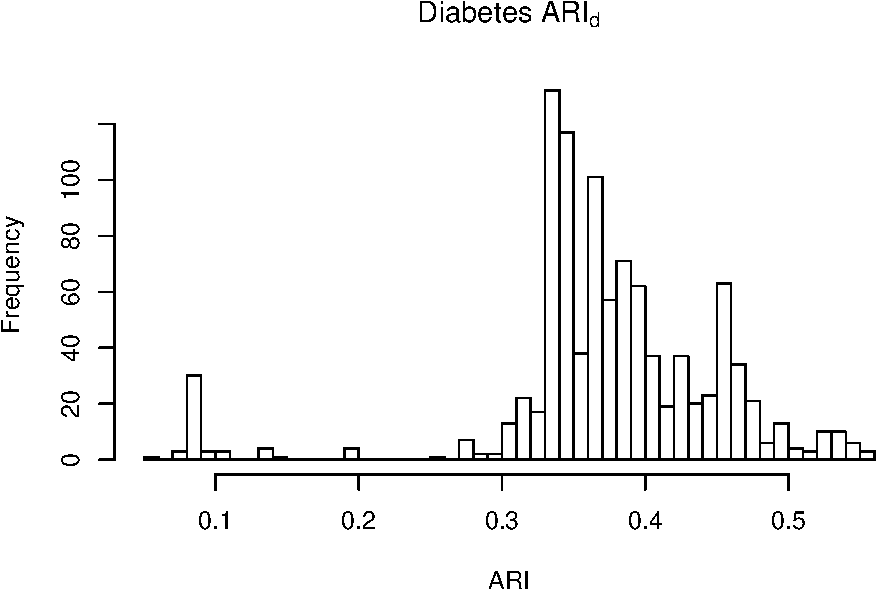
\includegraphics[width=1\linewidth]{Report_files/figure-latex/unnamed-chunk-18-3} \end{center}

\begin{center}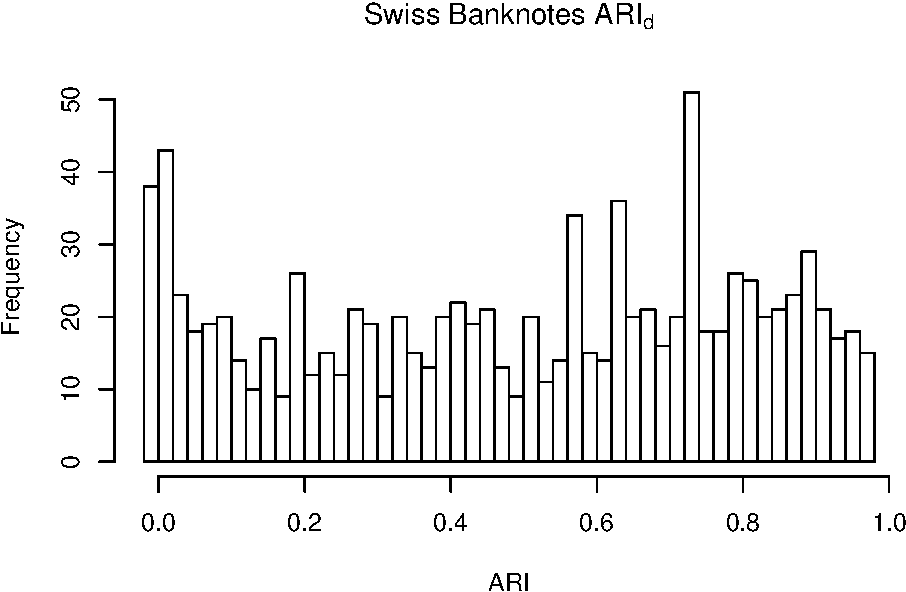
\includegraphics[width=1\linewidth]{Report_files/figure-latex/unnamed-chunk-18-4} \end{center}

\begin{center}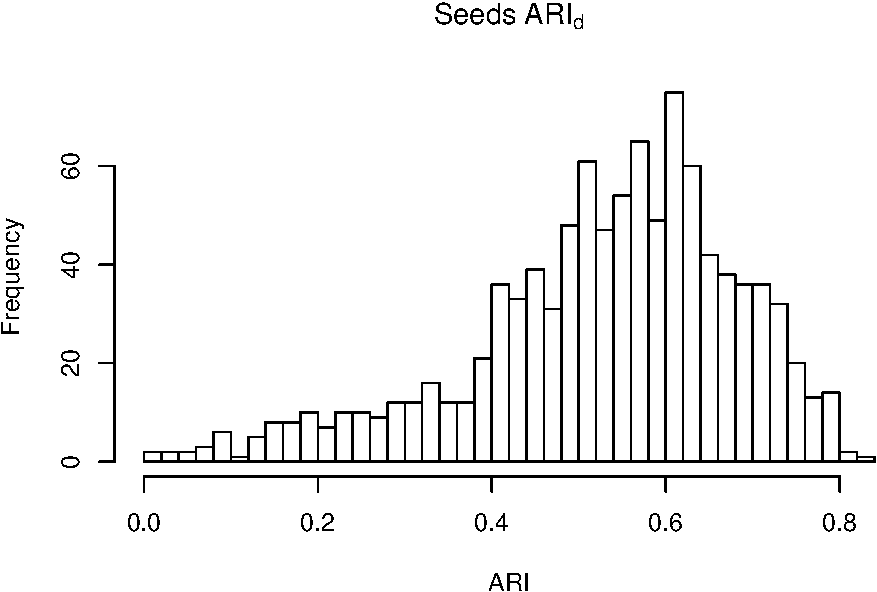
\includegraphics[width=1\linewidth]{Report_files/figure-latex/unnamed-chunk-18-5} \end{center}

\begin{center}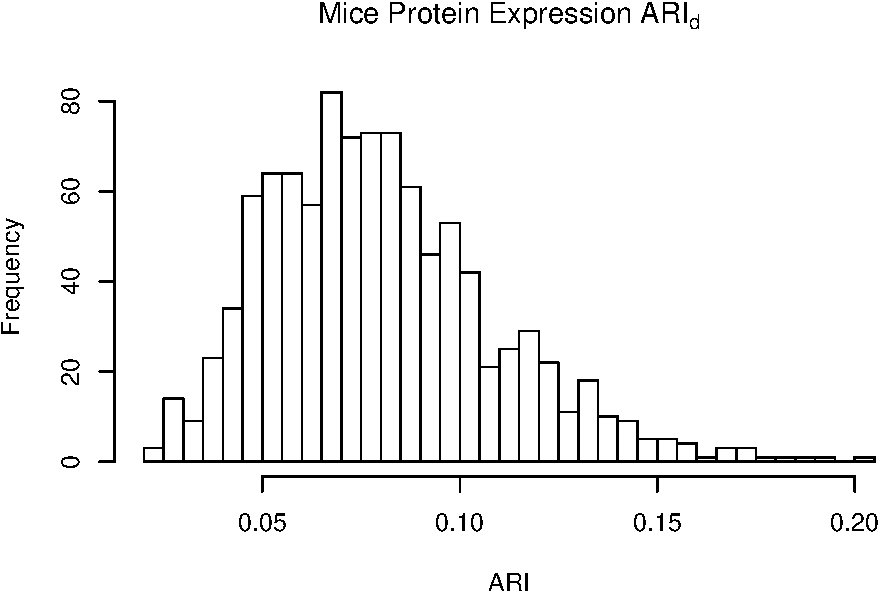
\includegraphics[width=1\linewidth]{Report_files/figure-latex/unnamed-chunk-18-6} \end{center}

\begin{center}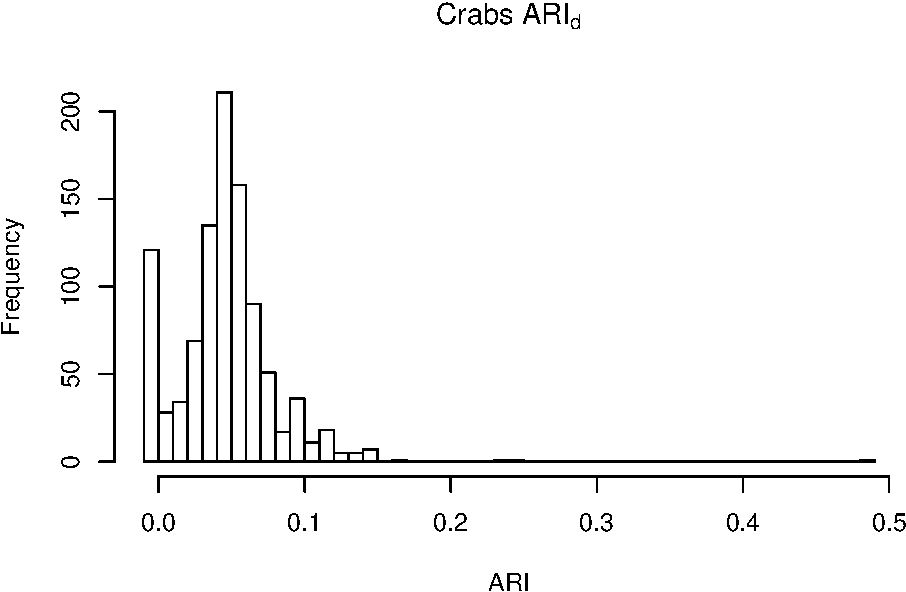
\includegraphics[width=1\linewidth]{Report_files/figure-latex/unnamed-chunk-18-7} \end{center}



\section{
بررسی تابعیت عملکرد کاهش بعد $C_e$ به ازای تغییر $\alpha$ برای کاهش بعد به دو بعد
}


\begin{center}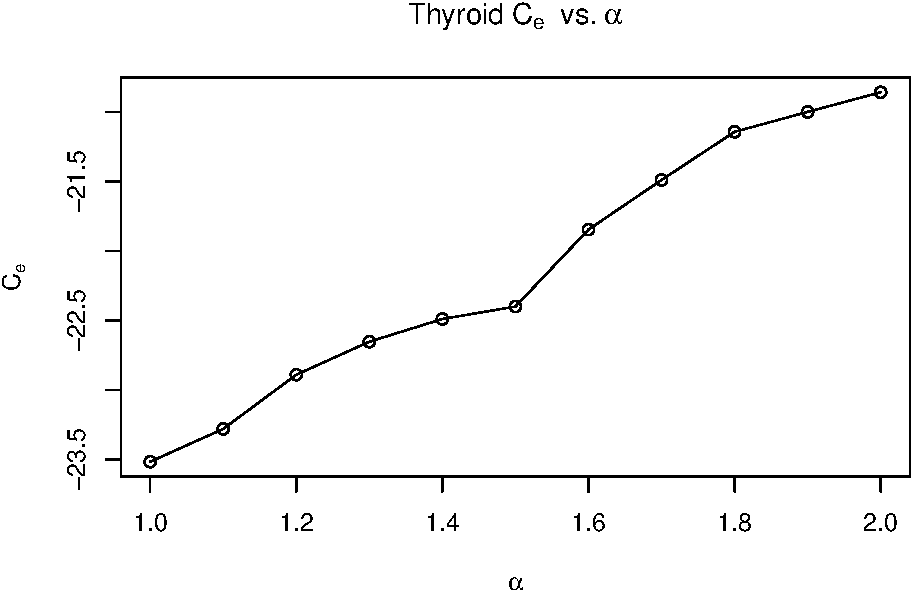
\includegraphics[width=1\linewidth]{Report_files/figure-latex/unnamed-chunk-20-1} \end{center}

\begin{center}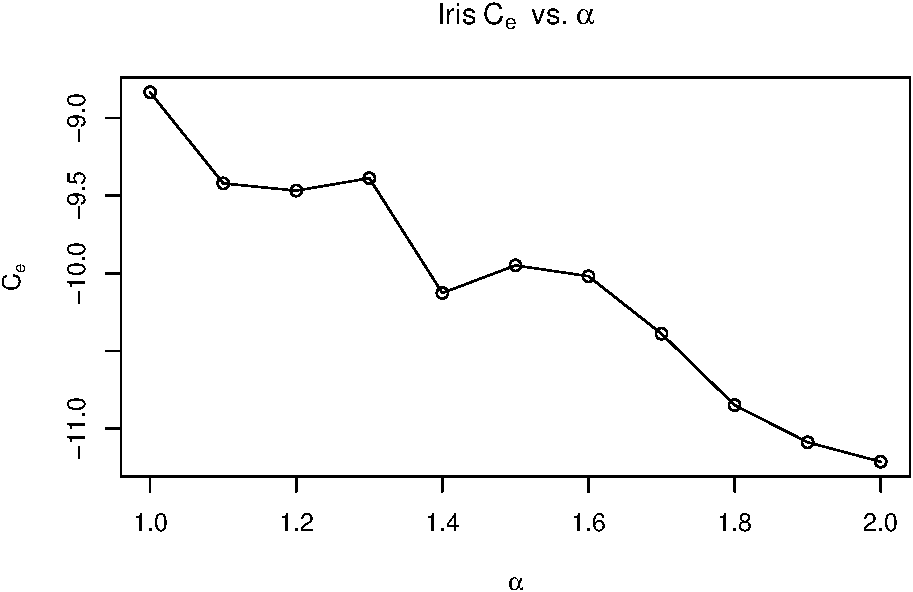
\includegraphics[width=1\linewidth]{Report_files/figure-latex/unnamed-chunk-20-2} \end{center}

\begin{center}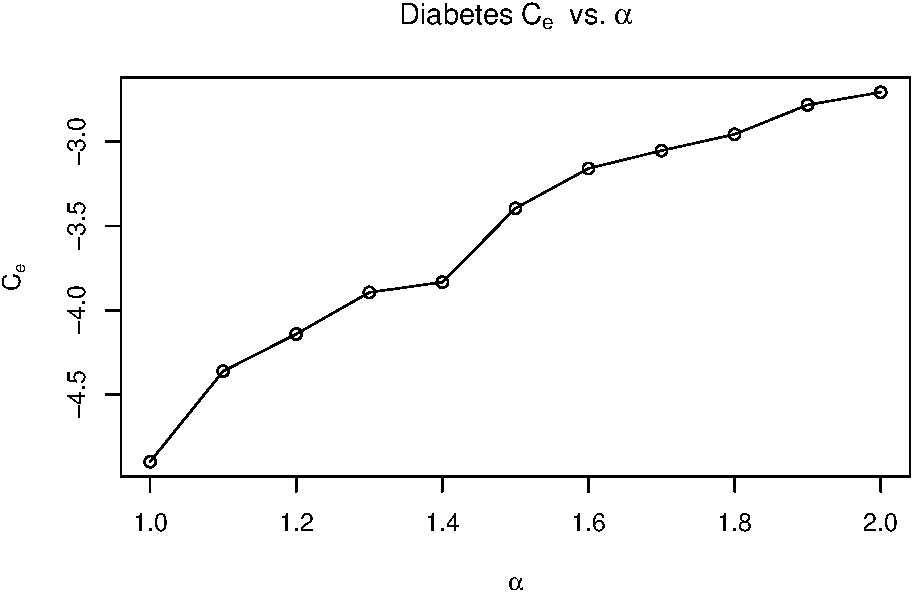
\includegraphics[width=1\linewidth]{Report_files/figure-latex/unnamed-chunk-20-3} \end{center}

\begin{center}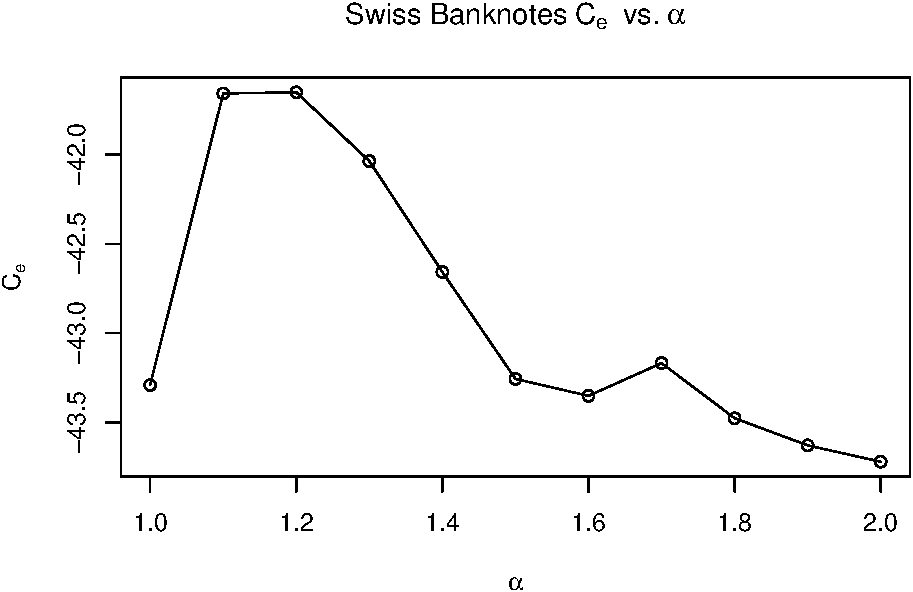
\includegraphics[width=1\linewidth]{Report_files/figure-latex/unnamed-chunk-20-4} \end{center}

\begin{center}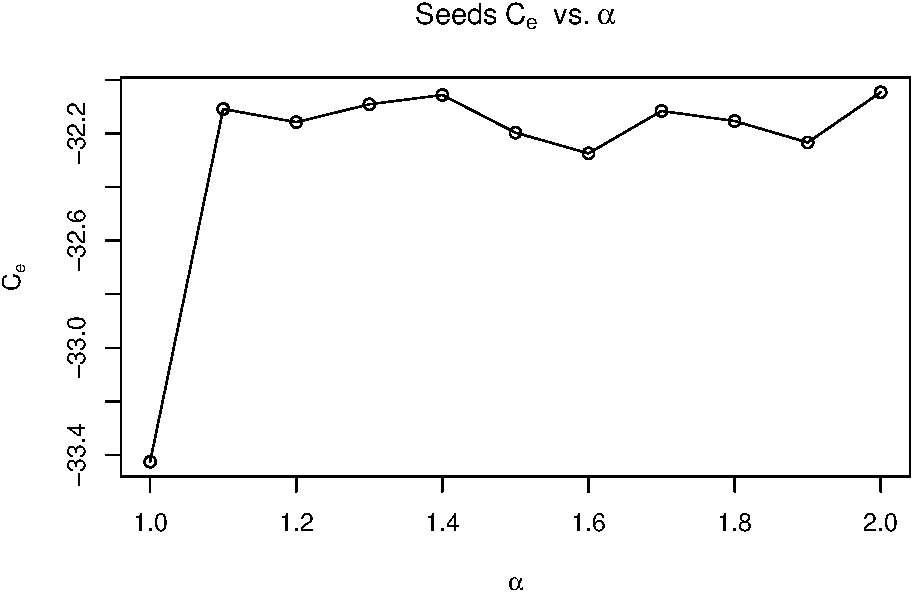
\includegraphics[width=1\linewidth]{Report_files/figure-latex/unnamed-chunk-20-5} \end{center}

\begin{center}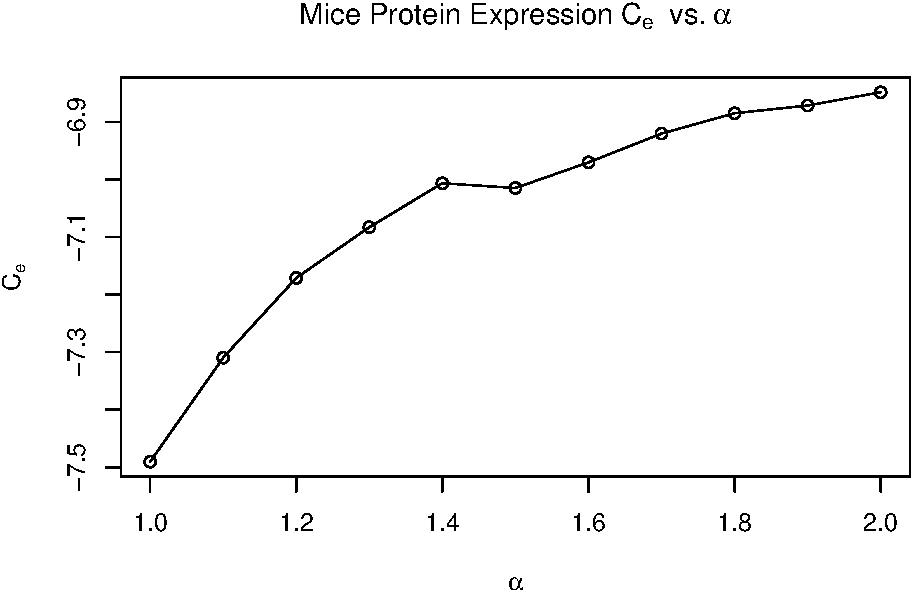
\includegraphics[width=1\linewidth]{Report_files/figure-latex/unnamed-chunk-20-6} \end{center}

\begin{center}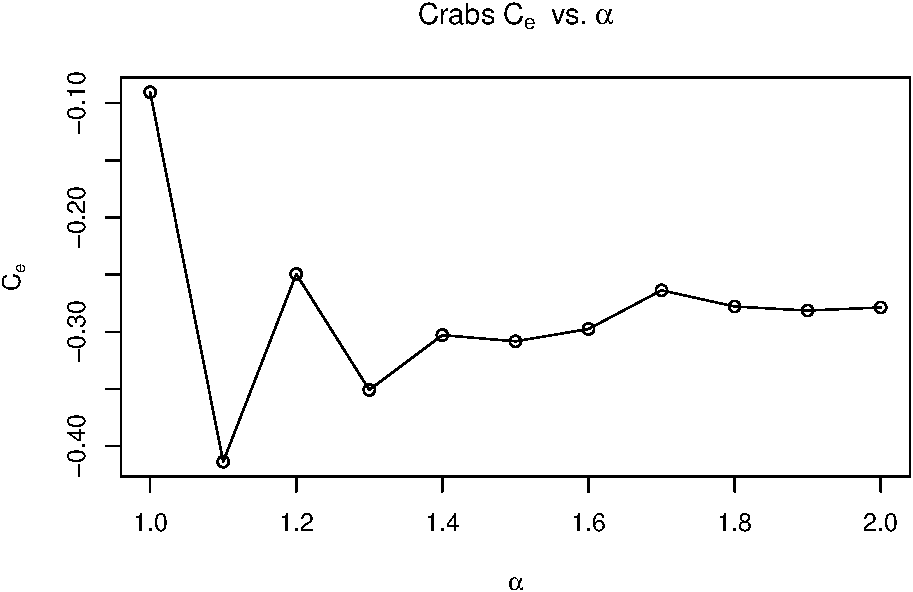
\includegraphics[width=1\linewidth]{Report_files/figure-latex/unnamed-chunk-20-7} \end{center}



\section{
بررسی تابعیت عملکرد کاهش بعد $C_e$ به ازای تغییر $\alpha$ برای کاهش بعد به سه بعد
}


\begin{center}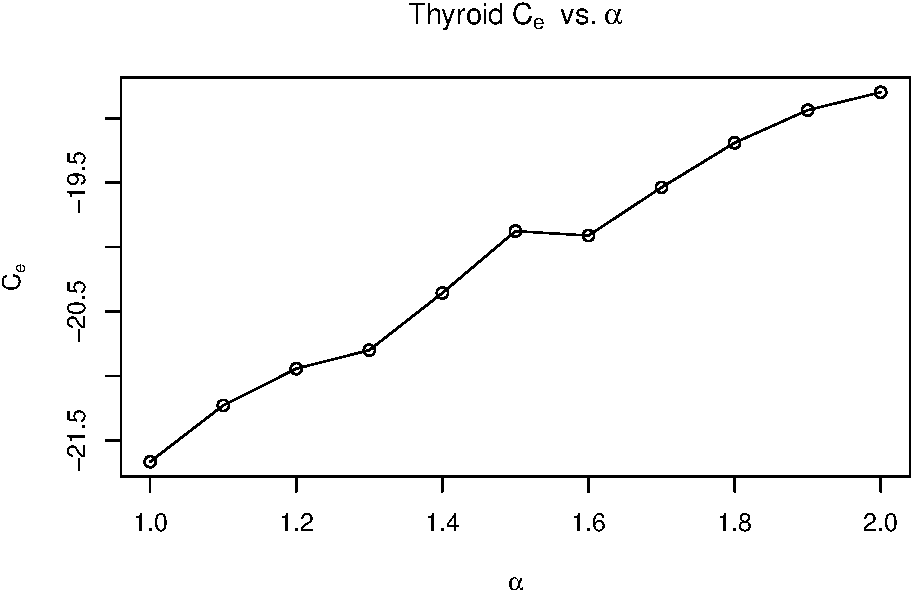
\includegraphics[width=1\linewidth]{Report_files/figure-latex/unnamed-chunk-22-1} \end{center}

\begin{center}\includegraphics[width=1\linewidth]{Report_files/figure-latex/unnamed-chunk-22-2} \end{center}

\begin{center}\includegraphics[width=1\linewidth]{Report_files/figure-latex/unnamed-chunk-22-3} \end{center}

\begin{center}\includegraphics[width=1\linewidth]{Report_files/figure-latex/unnamed-chunk-22-4} \end{center}

\begin{center}\includegraphics[width=1\linewidth]{Report_files/figure-latex/unnamed-chunk-22-5} \end{center}

\begin{center}\includegraphics[width=1\linewidth]{Report_files/figure-latex/unnamed-chunk-22-6} \end{center}

\begin{center}\includegraphics[width=1\linewidth]{Report_files/figure-latex/unnamed-chunk-22-7} \end{center}

\section{
بررسی تابعیت عملکرد کاهش بعد $C_e$ به ازای تغییر $s$ برای کاهش بعد گسسته به دو بعد
}


\begin{center}\includegraphics[width=1\linewidth]{Report_files/figure-latex/unnamed-chunk-24-1} \end{center}

\begin{center}\includegraphics[width=1\linewidth]{Report_files/figure-latex/unnamed-chunk-24-2} \end{center}

\begin{center}\includegraphics[width=1\linewidth]{Report_files/figure-latex/unnamed-chunk-24-3} \end{center}

\begin{center}\includegraphics[width=1\linewidth]{Report_files/figure-latex/unnamed-chunk-24-4} \end{center}

\begin{center}\includegraphics[width=1\linewidth]{Report_files/figure-latex/unnamed-chunk-24-5} \end{center}

\begin{center}\includegraphics[width=1\linewidth]{Report_files/figure-latex/unnamed-chunk-24-6} \end{center}

\begin{center}\includegraphics[width=1\linewidth]{Report_files/figure-latex/unnamed-chunk-24-7} \end{center}


\section{
بررسی تابعیت عملکرد کاهش بعد $C_e$ به ازای تغییر $s$ برای کاهش بعد گسسته به سه بعد
}


\begin{center}\includegraphics[width=1\linewidth]{Report_files/figure-latex/unnamed-chunk-26-1} \end{center}

\begin{center}\includegraphics[width=1\linewidth]{Report_files/figure-latex/unnamed-chunk-26-2} \end{center}

\begin{center}\includegraphics[width=1\linewidth]{Report_files/figure-latex/unnamed-chunk-26-3} \end{center}

\begin{center}\includegraphics[width=1\linewidth]{Report_files/figure-latex/unnamed-chunk-26-4} \end{center}

\begin{center}\includegraphics[width=1\linewidth]{Report_files/figure-latex/unnamed-chunk-26-5} \end{center}

\begin{center}\includegraphics[width=1\linewidth]{Report_files/figure-latex/unnamed-chunk-26-6} \end{center}

\begin{center}\includegraphics[width=1\linewidth]{Report_files/figure-latex/unnamed-chunk-26-7} \end{center}




